\hypersetup{colorlinks=true, linkcolor=blue, citecolor=red}

\chapter{Methodology} \label{chap:methodology}

    In this chapter, the methodology used to split data and train models is presented. In addition, the fundamental concepts behind the models used are explained.

    \section{Overview of the models}

        In this comparative study, a total of ten popular models are selected for analysis of their performance on Kinect skeleton data.

        \subsection{Scikit-learn library}  

            Scikit-Learn is a Python library designed for Machine Learning, it offers a wide range of \textit{state of the art} algorithms for medium-scale supervised and unsupervised problems. It emphasizes ease of use, performance, and API consistency, targeting non-specialists with its high-level approach. It stands out for its minimal dependencies and broad accessibility, being distributed under the simplified BSD license. It integrates well with the Python ecosystem, making it highly desirable for both academic and commercial applications \cite{scikit-learn}.

        \subsection{Models selection}

        Models presented in Table \ref{tab:movements_table} are used for a classification task. Selected based on popularity and performance, these models are widely used in the Machine Learning community. Models are implemented using \textit{Scikit-Learn} library and its functions for training, testing, and evaluating \cite{sklearn_api}. 

        \newpage 

        \begin{table}[htbp]
            \centering
            \begin{tabular}{@{}clcl@{}}
                \toprule
                \multicolumn{4}{c}{\textbf{Model Name}} \\
                \midrule
                1 & Support Vector Machine & 6 & Linear Discriminant Analysis \\
                2 & Gaussian Naive Bayes & 7 & Multi-Layer Perceptron \\
                3 & Random Forest & 8 & K Nearest Neighbors \\
                4 & Gradient Boosting & 9 & AdaBoost \\
                5 & Logistic Regression & 10 & Decision Tree \\
                \bottomrule
            \end{tabular}
            \caption{Models selected for use in this thesis.}
            \label{tab:movements_table}
        \end{table}
    
    \section{Models analysis}
        
        In this section models that performed best in Chapter \ref{chap:results_and_discussion} are analyzed in terms of their implementation.

        \subsection{Random forest}
           Also known as \textit{random decision forests}, it is a method of ensemble learning used for classification, regression, and various other tasks. It involves building numerous decision trees during a training phase. In classification tasks, the class chosen by a majority of trees is an output of the random forest \cite{ho_random_1998}.

           \begin{figure}[H]
            \centering
            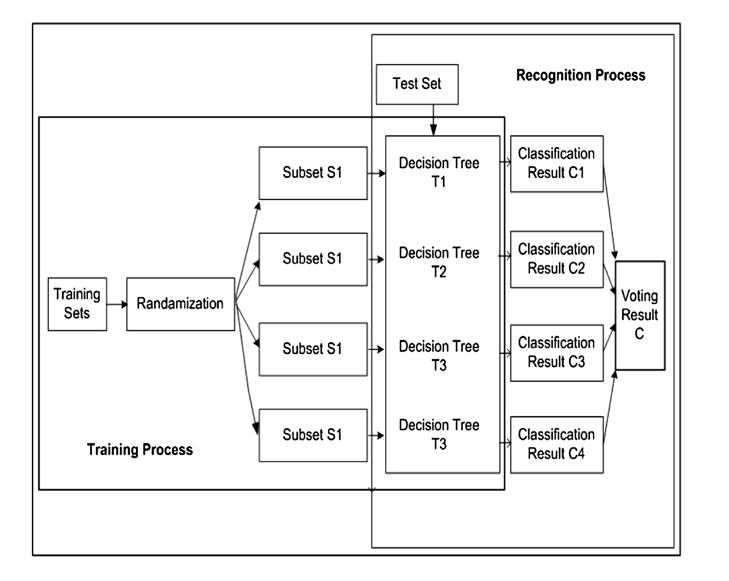
\includegraphics[width=.7\textwidth]{../src/resources/images/models/rf_image.png}
            \caption{
                The process starts with multiple training sets that undergo randomization to create several subsets S1. Each subset is used to train a separate decision tree (T1 to T3). Trained trees are then used to make predictions on a test set. Predictions (C1 to C4) from each tree are aggregated through a voting mechanism to produce a final classification result (C). This ensemble approach leverages multiple models to improve prediction accuracy and robustness \cite{parmar_review_2019}.
            }
            \label{fig:random_forest}
            \end{figure}

            The main steps involved in building a random forest classifier are as follows:
           
            \begin{enumerate}
                \item Define $M$ as the number of features in each subset.
                \item Randomly select a feature subset $\theta_k$ from the full set, distinct from proceding subset $\theta_{1},..., \theta_{k-1}$.
                \item Train decision trees on each $\theta_k$ denoted as $h(X, \theta_k)$.
                \item Iteratively select new $\theta_k$ subsets and train until all trees are built.
                \item Classify test data by majority vote of all trees in the forest.
            \end{enumerate}

            Random Forests consist of numerous decision trees. Randomization in tree building through sampling instances and feature subsets via bagging enhances diversity, reducing overfitting and improving generalization. Feature subsets $\theta_k$​ are chosen by bagging, and the importance of features is ranked by their impact on the model's accuracy "strength" and "correlation" of the forest are influenced by $M$, with optimal values providing a balance. Random forests efficiency is due to its parallel structure, accelerating classification significantly \cite{parmar_review_2019}.
            
        \subsection{Gradient boosting}
            Gradient Boosting is a Machine Learning method that refines predictions iteratively, combining strengths of simple models, like decision trees, into a more accurate ensemble. Each iteration, represented by $F_m(x)$, improves upon the last by adding a weighted decision tree $\rho_m h_m(x)$ that addresses the previous errors. The process follows the \textit{principle of gradient descent}, where $h_m(x)$ is trained to predict the negative gradient of a loss function, effectively reducing residual between the predicted and true values. Ensemble begins with a single model $F_0(x)$, which is updated by the formula:
            \begin{equation}
                F_m(x) = F_{m-1}(x) + \rho_m h_m(x)
            \end{equation}
            The aim is to minimize loss function $L(y, F_m(x))$ at each step, ensuring the model's prediction becomes progressively more accurate \cite{bentejac_comparative_2021}.
            \begin{figure}[H]
                \centering
                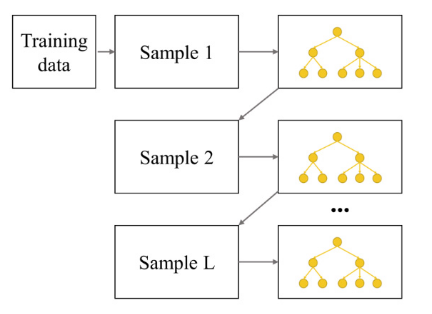
\includegraphics[width=.5\textwidth]{../src/resources/images/models/boosting.png}
                \caption{
                    Starting with training data, an algorithm iteratively trains decision trees (Sample 1 to Sample L). Each tree is trained on errors of the previous ones, aiming to correct these mistakes. Over multiple iterations, each tree improves the model's predictions, and the final output is a combined effort of all trees, effectively reducing prediction errors \cite{cha_comparison_2021}.
                }
                \label{fig:gradient_boosting}
            \end{figure}

        \newpage

        \subsection{Logistic regression}
            Logistic Regression is a statistical model used for binary classification that predicts the probability of a binary response based on one or more predictor variables. It applies a logistic function to a linear combination of input features to produce a value between 0 and 1, interpreted as A probability of the instance being in a positive class.
            Equation \ref{eq:logistic_regression} shows the logistic function for binary classification.

            \begin{equation} \label{eq:logistic_regression}
                P(Z) = \frac{1}{1 + e^{-(\beta_0 + \beta_1 x)}}
            \end{equation}

            In multi-class classification, the one vs rest approach involves training a separate logistic regression classifier for each class to distinguish that class from all other classes. For each classifier, the class is designed to identify as the positive class, and all others are lumped into a single negative class.
            The logistic function is the same as for binary classification, presented in Equation \ref{eq:logistic_regression}. It is applied multiple times, one for each class.
            
            \begin{figure}[htbp]
                \centering
                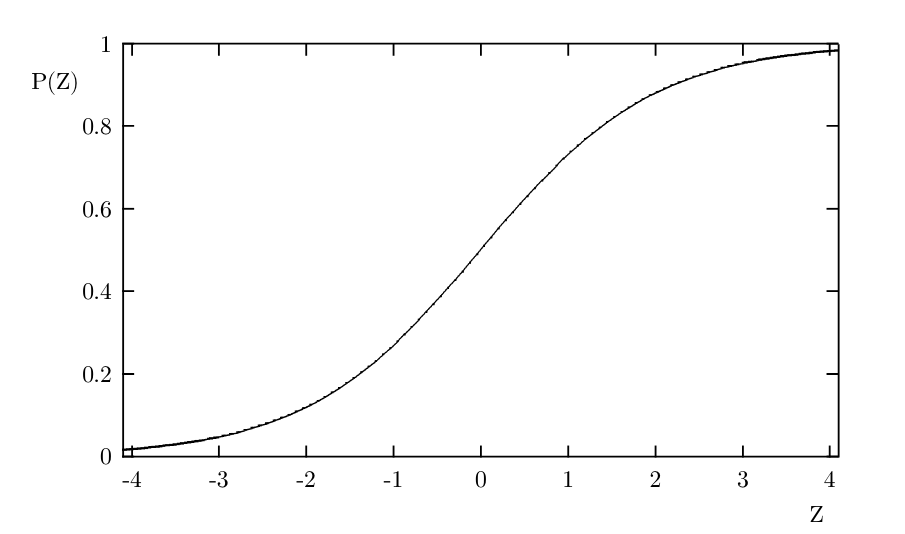
\includegraphics[width=.8\textwidth]{../src/resources/images/models/logistic.png}
                \caption{
                    The horizontal axis labeled \textit{Z} represents an input variable (which is a linear combination of the features), and the vertical axis labeled \textit{P(Z)} represents a probability that an outcome is a positive class. The curve transitions smoothly from 0 to 1, with an inflection point at Z=0, where P(Z) = 0.5. This S-shaped curve allows logistic regression to convert continuous predictions into a probability between 0 and 1, facilitating binary classification \cite{cramer_origins_2002}.
                }
                \label{fig:logistic_regression}
            \end{figure}

        \subsection{Linear discriminant analysis}
            Linear Discriminant Analysis (LDA) is a method used in Statistics and Machine Learning to find a linear combination of features that separates two or more classes of objects or events. It does so by maximizing a ratio of between-class variance to a within-class variance in any particular data set, thereby ensuring maximum separability.

            In a binary class, the goal is to find a linear combination $w$ that separates the classes. This involves computing mean vectors $m_1$ and $m_2$ for each class, within-class scatter matrix $S_W$, and between-class scatter matrix $S_B$. Linear discriminants are then the eigenvectors of $S_W^{-1}S_B$ \cite{xanthopoulos_linear_2013}. 

            \begin{figure}[H]
                \centering
                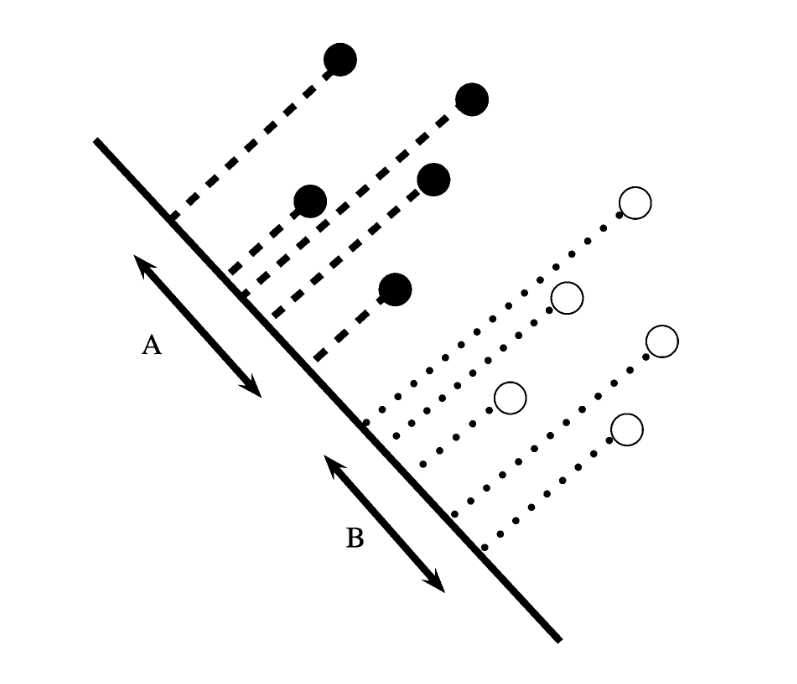
\includegraphics[width=.6\textwidth]{../src/resources/images/models/lda.png}
                \caption{
                    The intuition behind LDA. Data samples in two dimensions are projected in a lower-dimension space. The line has to be chosen so that the projection maximizes the "separability" of projected samples \cite{xanthopoulos_linear_2013}.
                }
                \label{fig:linear_discriminant_analysis}
            \end{figure}

            For multi-class problems, the same principle applies but extends to multiple classes. Within class scatter matrix $S_W$ and between class scatter matrix $S_B$ are computed considering all classes, and the objective is to find linear discriminants that maximize separation among all classes.  

            The simplicity and effectiveness of LDA, especially under assumptions of normality and equal class covariances, make it a powerful tool for classification \cite{balakrishnama_linear_nodate}.

        \subsection{Multi layer perceptron}
            Multi Layer Perceptron architecture includes at least three layers, an input layer, an output layer, and one or more hidden layers, each composed of nodes with non-linear activation functions \cite{svozil_introduction_1997}. They are referred to as "vanilla" neural networks \cite{hastie_elements_2009}.

        \begin{equation}\label{eq:tan}
            y(v_i) = \text{tanh}(v_i) 
        \end{equation}

        \begin{equation}\label{eq:sigmoid}
            y(v_i) = (1+e^{-v_i})^{-1} 
        \end{equation}

            A linear function can simplify multiple layers to a two-layer model, mapping weighted inputs to neuron outputs. Non-linear activation functions, like hyperbolic tangent \ref{eq:tan} ranging from -1 to 1, or sigmoid function \ref{eq:sigmoid} ranging from 0 to 1, are used to introduce non-linearity into a model. This allows a model to learn complex patterns in the data.

        \newpage

        In the context of MLP, complete connectivity is maintained, every node within a given layer connects to every node in the subsequent layer via weighted connections. \\
        The learning process involves dynamic adjustment of connection weights following the processing of each data point. This adjustment is made in response to the disparity between actual output and expected outcome, to minimize error.

        \begin{figure}[H]
            \centering
            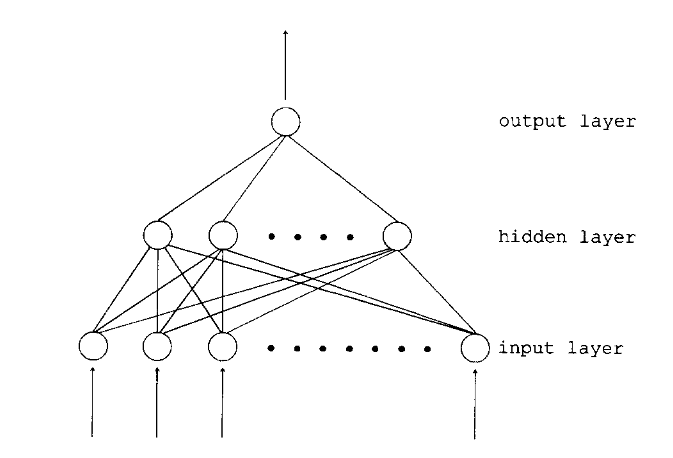
\includegraphics[width=.7\textwidth]{../src/resources/images/models/feedforward.png}
            \caption{
                Feed-forward network consists of an input layer, one or more hidden layers, and an output layer \cite{svozil_introduction_1997}.
            }
            \label{fig:multi_layer_perceptron}
        \end{figure}
    
    \newpage
        
        
    \section{Data splitting methods}
        
            Due to the structure of data, a traditional approach of splitting data into training and testing sets is not effective. Two different approaches will be presented, one ineffective and one effective.

            \subsection{Traditional} \label{sec:badsplit}
                        
                    Data is split into 70\% training and 30\% testing following a traditional approach used in Machine Learning literature. The code snippet in \ref{lst:badsplit} demonstrates this approach. 
            
\begin{lstlisting}[
    caption={Traditional approach to splitting data into training and testing sets.}, 
    label={lst:badsplit},
    ]            
    def split_data(data: pd.DataFrame) -> tuple:        
        X = data.iloc[:, :-1].values
        y = data.iloc[:, -1].values
        
        X_train, X_test, y_train, y_test = train_test_split(
            X, y, test_size=0.33, random_state=42)
        
        return X_train, X_test, y_train, y_test
\end{lstlisting}
                
                    Figure \ref{fig:badsplit} visualization demonstrates why this approach is ineffective. Every row in the dataset is associated with a specific patient. Data is split randomly, so there is a chance that the same patient will appear in both training and testing sets. This means that a model will be trained on data that it will also be tested on, which will result in a high accuracy score. However, this is not a good indicator of a model's performance on unseen data.

                    \begin{figure}[H]
                        \centering
                        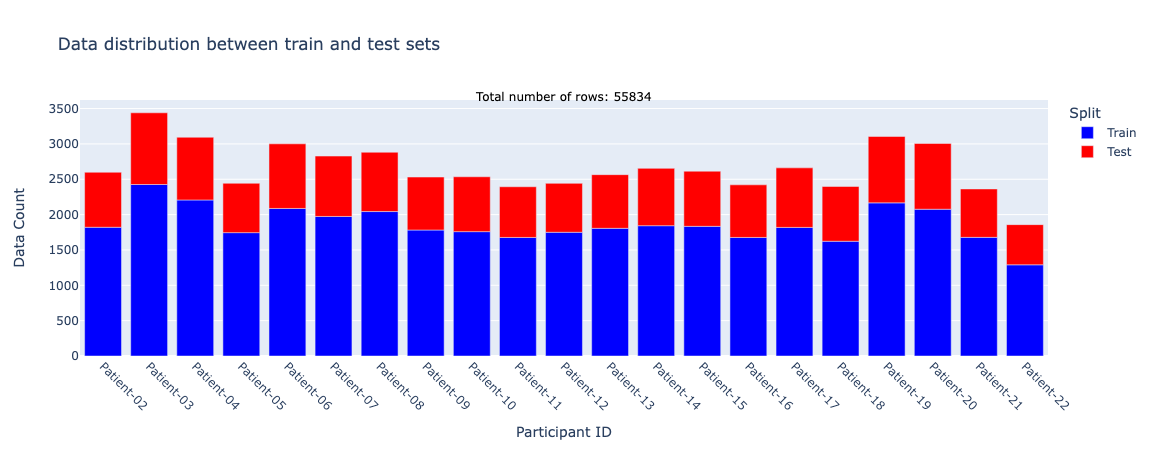
\includegraphics[width=1.0\textwidth]{../src/resources/plots/splits/bad.png}
                        \caption{
                            patient presence in both training and testing sets visualization.
                        }
                        \label{fig:badsplit}
                    \end{figure}
        
                    \newpage

            \subsection{Effective} \label{sec:goodsplit}
            Data is split into training and testing sets based on a patient's unique IDs. They are split into training and testing sets, and then data is split based on patient's unique ids. The code snippet in \ref{lst:goodsplit} demonstrates this approach.

\begin{lstlisting}[
    caption={Effective approach to splitting data into training and testing sets.}, 
    label={lst:goodsplit}]
    def split_data(data: pd.DataFrame) -> tuple:    
        unique_patient = data['patient'].unique()

        train_patients, test_patients = train_test_split(unique_patients, test_size=0.3, random_state=42)

        train_data = data[data['patient'].isin(train_patients)]
        test_data = data[data['patient'].isin(test_patients)] 

        X_train = train_data.drop(columns=['label', 'patient'])
        y_train = train_data['label']

        X_test = test_data.drop(columns=['label', 'patient'])
        y_test = test_data['label']
        
        return X_train, X_test, y_train, y_test
\end{lstlisting}

            Figure \ref{fig:goodsplit} visualization demonstrates why this approach is effective. Data is split based on patients' unique IDs, so a model will be trained on data that will not be tested. This means that a model will be tested on unseen data, which is a good indicator of a model's performance.

            \begin{figure}[H]
                \centering
                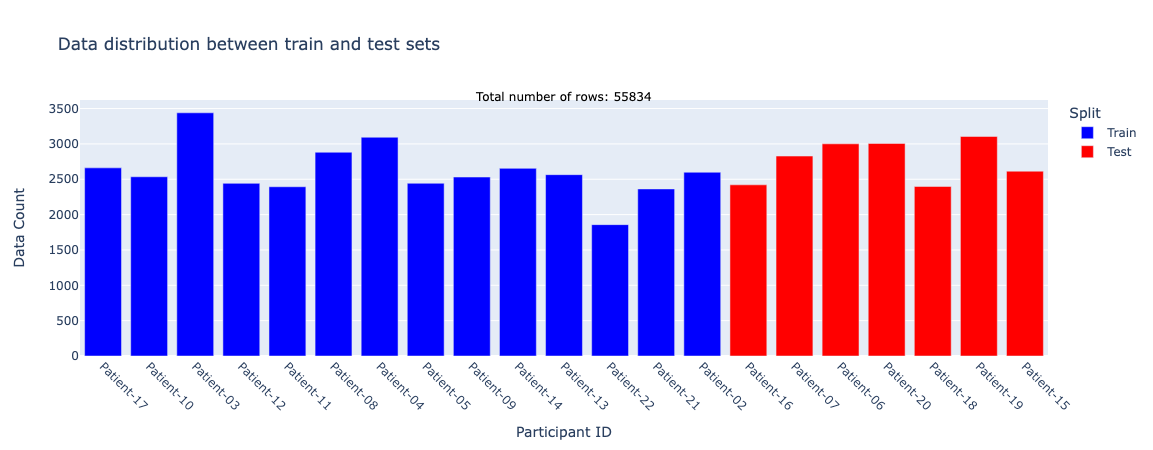
\includegraphics[width=1.0\textwidth]{../src/resources/plots/splits/good.png}
                \caption{
                    Patients split between training and testing sets visualization, ensuring that a patient is only present in one of the sets.
                }
                \label{fig:goodsplit}
            \end{figure}

    \newpage
            
            \subsection{Sequential} \label{sec:seqsplit}
            Data is split into training and testing sets based on the patient's unique IDs, then sets are split into sequences. Where each sequence represents a stack of frames that make up a movement. The code snippet in \ref{lst:seqsplit} demonstrates this splitting technique. 

\begin{lstlisting}[
    caption={Effective approach to splitting data into training and testing sets.}, 
    label={lst:seqsplit}]                
    def sequences(df: pd.DataFrame, feature_columns: list, sequence_column: str) -> tuple:
        sequences = []
        labels = []
        current_sequence = []
        current_check = None

        for _, row in df.iterrows():
            check = row[sequence_column]
            label = row['label']
            if check != current_check and current_sequence:
                sequences.append(np.array(current_sequence))
                labels.append(label)
                current_sequence = []
            current_sequence.append(row[feature_columns].to_numpy())
            current_check = check

        if current_sequence: 
            sequences.append(np.array(current_sequence))
            labels.append(label)

        return sequences, labels
\end{lstlisting}

            Figure \ref{fig:seqsplit} visualization shows how for each movement data is split into sequences for training and testing. However, using only this approach is not enough, as the sequences are of different lengths due to each movement having a variable number of frames. This means that sequences cannot be used as input for models since they require a fixed input size. 
        
            \begin{figure}[H]
            \centering
            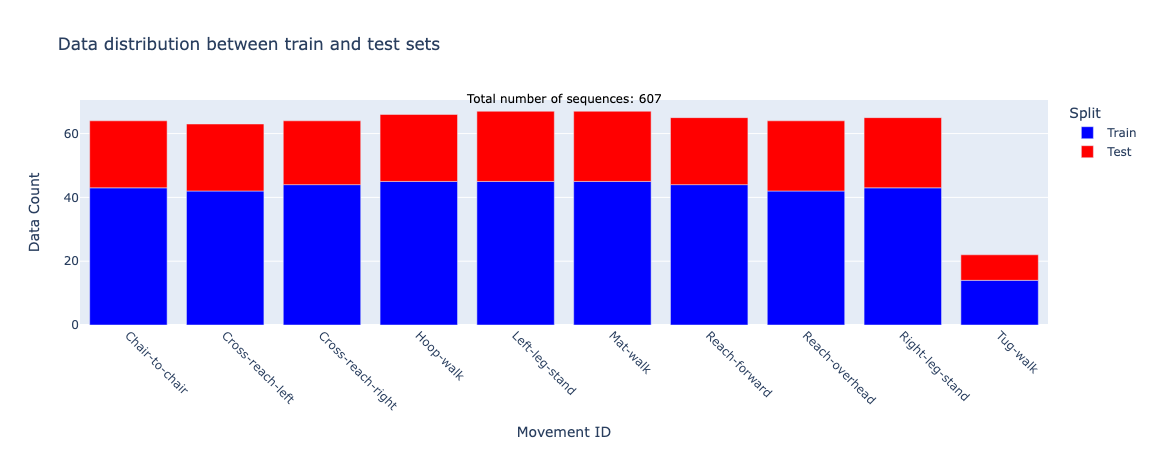
\includegraphics[width=1.0\textwidth]{../src/resources/plots/splits/seq.png}
            \caption{
                Visualization of the sequences splitting approach.
            }
            \label{fig:seqsplit}
        \end{figure}

        \newpage 

        To solve this variable length problem, sequences are aggregated into a single feature vector. Code snippet \ref{lst:seqagg} demonstrates this approach. In Figure \ref{fig:seqlength}, the length of sequences before and after aggregation is visualized. Aggregation is done by calculating the mean of each feature for each frame in the sequence. This results in a single feature vector for each sequence, which can be used as input for the models.

\begin{lstlisting}[
    caption={Sequences are aggregated into a single feature vector.}, 
    label={lst:seqagg}]                
    def aggregate_features(sequences: list) -> np.ndarray:
            return np.array([np.mean(sequence, axis=0) if sequence.size != 0 else np.zeros(sequence.shape[1]) for sequence in sequences])
\end{lstlisting}
        
However, there are some drawbacks to this approach. The aggregation results in a loss of information, as data is no longer represented as a sequence of frames. In addition, aggregation results in a loss of temporal information, as the order of frames is lost. This means that models will not be able to learn temporal patterns in data.

\begin{figure}[H]
    \centering
    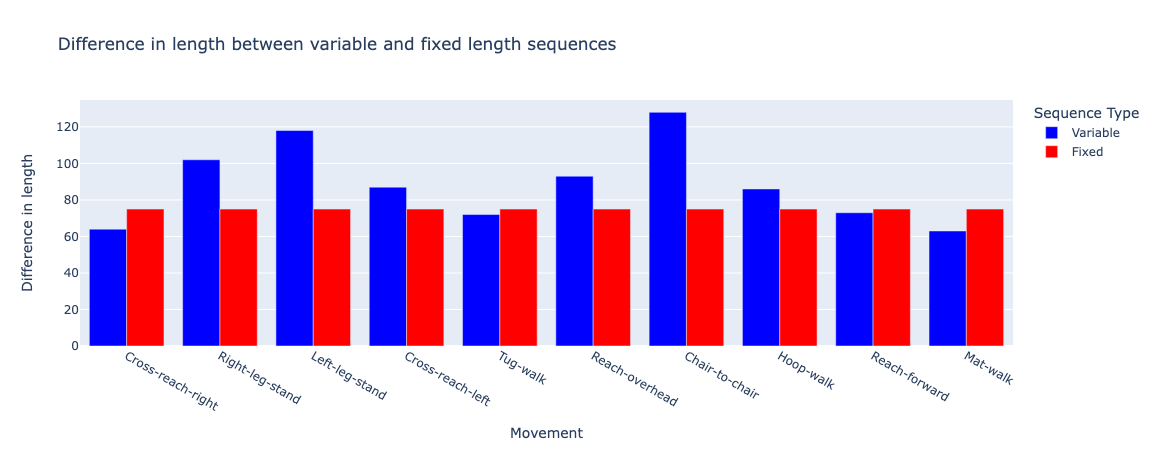
\includegraphics[width=1.0\textwidth]{../src/resources/plots/splits/seq_len.png}
    \caption{
        Visualization of the length of the sequences before and after aggregation.
    }
    \label{fig:seqlength}
\end{figure}

    \newpage
    
    \section{Feature engineering} \label{sec:feature_engineering}
        
        Feature engineering is the final approach used in this thesis. It is used to extract new features from raw Kinect skeleton data, to improve the performance of the models.

        \subsection{Overview}

            This process is implemented to improve the performance of the models due to them not being able to differentiate well between movements based on raw data. This allows us to obtain data that is more informative and easier to interpret. Features extracted from Kinect skeleton data are presented in Table \ref{tab:features_table}.

        \begin{table}[htbp]
            \centering
            \begin{tabular}{@{}clcl@{}}
                \toprule
                \multicolumn{4}{c}{\textbf{Features}} \\
                \midrule
                1 & Duration & 2 & Area \\
                3 & Velocity & 4 & Distance \\
                5 & Vertical displacement & 6 & Horizontal displacement \\
                7 & Forward displacement &  & \\
                \bottomrule
            \end{tabular}
            \caption{Features extracted from Kinect skeleton data.}
            \label{tab:features_table}
        \end{table}

        \subsection{Calculation Methods}

            Features presented in Table \ref{tab:features_table} are calculated using the following methods. For each feature, the method used to calculate it is presented, along with a brief description.

            \begin{table}[ht]
                \centering
                \begin{tabular}{@{}clcl@{}}
                    \toprule
                    \multicolumn{4}{c}{\textbf{Body parts selected}} \\
                    \midrule
                     Head & ShoulderLeft & ShoulderRight & SpineShoulder \\
                     SpineMid & SpineBase & ElbowLeft & ElbowRight \\
                     WristLeft & WristRight & HipLeft & HipRight \\
                     KneeLeft & KneeRight & AnkleLeft & AnkleRight \\
                    \bottomrule
                \end{tabular}
                \caption{Selected body parts from Kinect skeleton data joints.}
                \label{tab:body_parts_table}
            \end{table} 

            \subsubsection{Duration}

                Duration is defined as how long it takes for a movement to be performed from start to finish. It is calculated as a difference between maximum and minimum datetime column values. It is calculated in seconds.

                \begin{equation}\label{eq:duration}
                    \text{Duration} = (\text{{max\_datetime}} - \text{{min\_datetime}})
                \end{equation}
            
            \subsubsection{Area}

                The area is defined as an aggregate area of convex hulls formed by trajectories of selected body parts. It operates by extracting (x, y, z) coordinates for each specified body part, constructing a convex hull for these points, and then calculating the hull's volume.

                \begin{equation}\label{eq:area}
                    \text{Area} = \sum_{i=0}^{n} \text{Volume}(\text{Hull}(P_i))
                \end{equation}
            
                In Equation \ref{eq:area}, $P_i$ is a set of points representing trajectory of body part $i$ in 3D space, where $i \in \{1, 2, ..., n\}$ for $n$ body parts. The Convex hull of $P_i$ is denoted as $\text{Hull}(P_i)$, which is the smallest convex set that contains all points in $P_i$. Volume (area in 3D) of $\text{Hull}(P_i)$ is calculated using a formula for the volume of a convex polyhedron, which depends on the vertices of the hull. The total area calculated is a sum of the volumes of these convex hulls for specified body parts.
                
        \begin{lstlisting}[caption={Area calculation method using ConvexHull class from SciPy library.}] 
        def area(df: pd.DataFrame, body_parts: list) -> float:
            def calculate(points: np.ndarray) -> float:
                hull = ConvexHull(points)
                return hull.volume
            trajectories = {}
            for column in body_parts:
                body_part = column.split('.')[0]
                trajectory = df[[body_part + '.px', body_part + '.py', body_part + '.pz']].values
                trajectories[body_part] = trajectory
            temp = {}
            for body_part, trajectory in trajectories.items():
                temp[body_part] = calculate(trajectory)
            return sum(temp.values())
        \end{lstlisting}

                \begin{figure}[H]
                    \centering
                    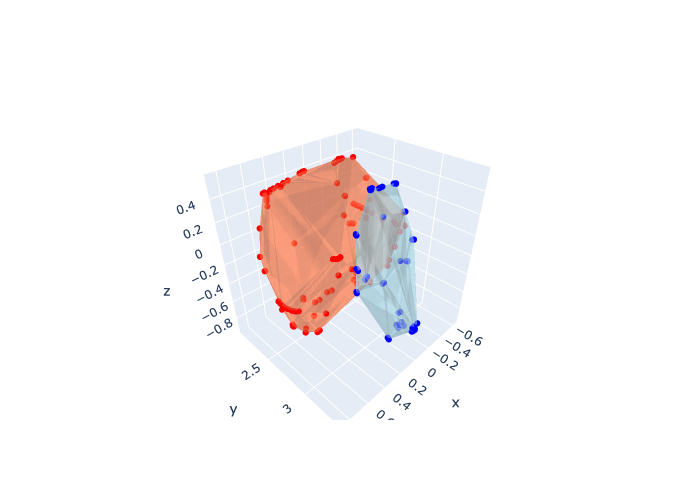
\includegraphics[width=.6\textwidth]{../src/resources/plots/feat-eng/area_difference.png}
                    \caption{
                        Visualization of the area occupied by two movements, red area represents \textit{Chair to Chair} while blue area represents \textit{Right Leg Stand}. 
                    }
                    \label{fig:area}
                \end{figure}
            
            \subsubsection{Velocity}
                
                Velocity is defined as a rate of change of displacement over time. It is calculated as the square root of the sum of squared displacement over time difference for each axis. 

                \begin{equation}\label{eq:velocity}
                    \text{velocity} = \sqrt{\left(\frac{\text{displacement}_x}{\text{time difference}}\right)^2 + \left(\frac{\text{displacement}_y}{\text{time difference}}\right)^2 + \left(\frac{\text{displacement}_z}{\text{time difference}}\right)^2}
                \end{equation}

                               
        \begin{lstlisting}[
            caption={Velocity calculation method.}, 
            label={lst:vertical_displacement}],     
    def velocity(df: pd.DataFrame) -> float:
        first = df.iloc[0]
        last = df.iloc[20]
        start = first['datetime'].split('_')[1].split('.')[0]
        end = last['datetime'].split('_')[1].split('.')[0]
        diff = pd.to_datetime(end) - pd.to_datetime(start)
        velx = last['Head.px'] - first['Head.px'] / diff.total_seconds()
        vely = last['Head.py'] - first['Head.py'] / diff.total_seconds()
        velz = last['Head.pz'] - first['Head.pz'] / diff.total_seconds()
        return math.sqrt(velx**2 + vely**2 + velz**2)
        \end{lstlisting}

                \begin{figure}[H]
                    \centering
                    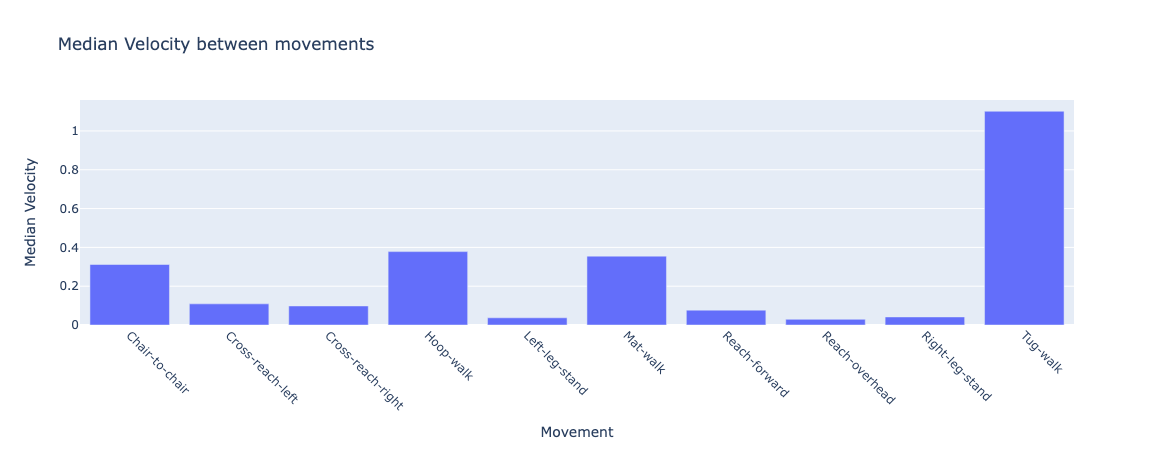
\includegraphics[width=1.0\textwidth]{../src/resources/plots/feat-eng/median_velocity.png}
                    \caption{
                       Visualization of the median velocity of each movement in the dataset. This shows how velocity varies between movements and can be used to differentiate between them.
                    }
                    \label{fig:velocity}
                \end{figure}

            \subsubsection{Distance}

                Distance is defined as the total 3D Euclidean distance between consecutive points representing a position of a body part, typically the head. It is calculated by taking each pair of consecutive rows in the dataset, computing the distance between their (x, y, z) head positions in 3D space using the Euclidean distance formula, and summing up these distances to find an overall total distance covered by a body part in the sequence.

                \begin{equation}
                    \text{Distance} = \sum_{i=0}^{n-1} \sqrt{(x_{i+1} - x_i)^2 + (y_{i+1} - y_i)^2 + (z_{i+1} - z_i)^2}
                \end{equation}

                \begin{lstlisting}[
                    caption={Distance calculation method.}, 
                    label={lst:vertical_displacement}],     
    def calculate(row1: pd.Series, row2: pd.Series, point="Head") -> float:
        return np.sqrt((row2[f'{point}.px'] - row1[f'{point}.px'])**2 +
                        (row2[f'{point}.py'] - row1[f'{point}.py'])**2 +
                        (row2[f'{point}.pz'] - row1[f'{point}.pz'])**2)
    
    def distance(df: pd.DataFrame) -> float:
        return sum(calculate(df.iloc[i], df.iloc[i+1]) for i in range(len(df) - 1))
                \end{lstlisting}
            \subsubsection{Time steps displacement}
                Following joints: \textit{AnkeLeft}, \textit{AnkleRight}, \textit{WristLeft}, \textit{WristRight}, \textit{SpineMid} have been selected for calculation of displacement. These joints have been selected as they are the most informative for the movements in the dataset. \\

                Time step displacement is defined as a total change in the position of a body part from the start to the end of a movement. It is calculated by taking absolute differences in positions of a body part between consecutive time steps, and then summing up these differences over all time steps.

                \begin{equation} \label{eq:displacement}
                    \text{Time steps displacement} = \sum_{t=1}^{n} \left| P(t) - P(t-1) \right|
                \end{equation}
                In Equation \ref{eq:displacement}, $P$ is a placeholder for axis positions of a body part, and $t$ is the time step. 
                \begin{enumerate}
                    \item \textbf{Vertical} is calculated by taking $Y$ axis positions.
                    \item \textbf{Horizontal} is calculated by taking $X$ axis positions.
                    \item \textbf{Forward} is calculated by taking $Z$ axis positions.
                \end{enumerate}
               
        \begin{lstlisting}[
    caption={Vertical time steps displacement calculation method.}, 
    label={lst:vertical_displacement}],     
    def vertical(df: pd.DataFrame, joint: str) -> float:
        df['vertical_diff'] = df[f'{joint}.py'].diff().abs()
        total_vertical = df['vertical_diff'].sum()
        return total_vertical
        \end{lstlisting}
\cleardoublepage
